\subsection{Android App}
\label{subsec:Software_App}

Um den Aufwand der Erstellung einer App möglichst gering halten zu können, wurde bei der Erstellung auf ein Web-Tool zurückgegriffen, welches mittels einer einfach gestalteten Benutzeroberfläche App-Erstellungen ermöglicht. Bei dem Programm handelt es sich um AppInventor. Es gibt einige weitere solche Anbieter wie auch Kodular. Bei diversen Programmierversuchen stellte sich jedoch heraus, dass AppInventor trotz einiger schwächen flüssiger und zuverlässiger läuft als seine Konkurrenz.  Die beiden grössten Schwächen von AppInventor sind, dass mit dem Tool keine dynamischen Buttons erstellt werden können, was es schwierig gestaltet Buttonlists oder ähnliches zu erstellen. Als weiterer grosser Schwachpunkt zählt, dass zwar verschiedene Seiten erstellt werden können, jedoch ein Bluetooth-Client zum Beispiel jeweils nur auf einer Seite aktiv sein kann. Somit müsste man bei einem Seitenwechsel jedes Mal den Bluetooth-Client neu verbinden. Beide Schwächen können jedoch mit einem Trick umgangen werden. Anstelle von Buttonlists oder dynamischen Schiebereglern kann man mit Dropdownisten arbeiten, welche sich bei der Öffnung jeweils aktualisieren und an Stelle eines Seitenwechsels kann mit der Sichtbarkeit von Elementen gearbeitet werden. Dies macht jedoch den Programmaufbau komplexer und unübersichtlicher. \cite{appinventor_mit_nodate} \cite{kodular_kodular_nodate} \\


AppInventor arbeitet mit zwei verschiedenen Benutzeroberflächen. Einerseits mit dem Designer, in welchem die App mit relativ einfachen Bausteinen gestaltet werden kann und anderseits mit den Blocks, wo der Programmablauf blockmässig erstellt werden kann.\\

Der Designer, welcher in Abbildung \ref{fig:AppInventorDesigner} zu sehen ist, besteht aus vier Einheiten. Ganz links befinden sich die Bausteine in der Palette, welche per Drag and Drop in den Viewer gezogen werden können, welcher sich gross in der Mitte befindet. Links neben dem Viewer befinden sich dann die schon rein gezogenen Komponenten als Übersicht und ganz rechts die Einstellungen und Formatierungsmöglichkeiten zu den gewählten Komponenten.

\newpage

\begin{figure}[h!]
	\centering
	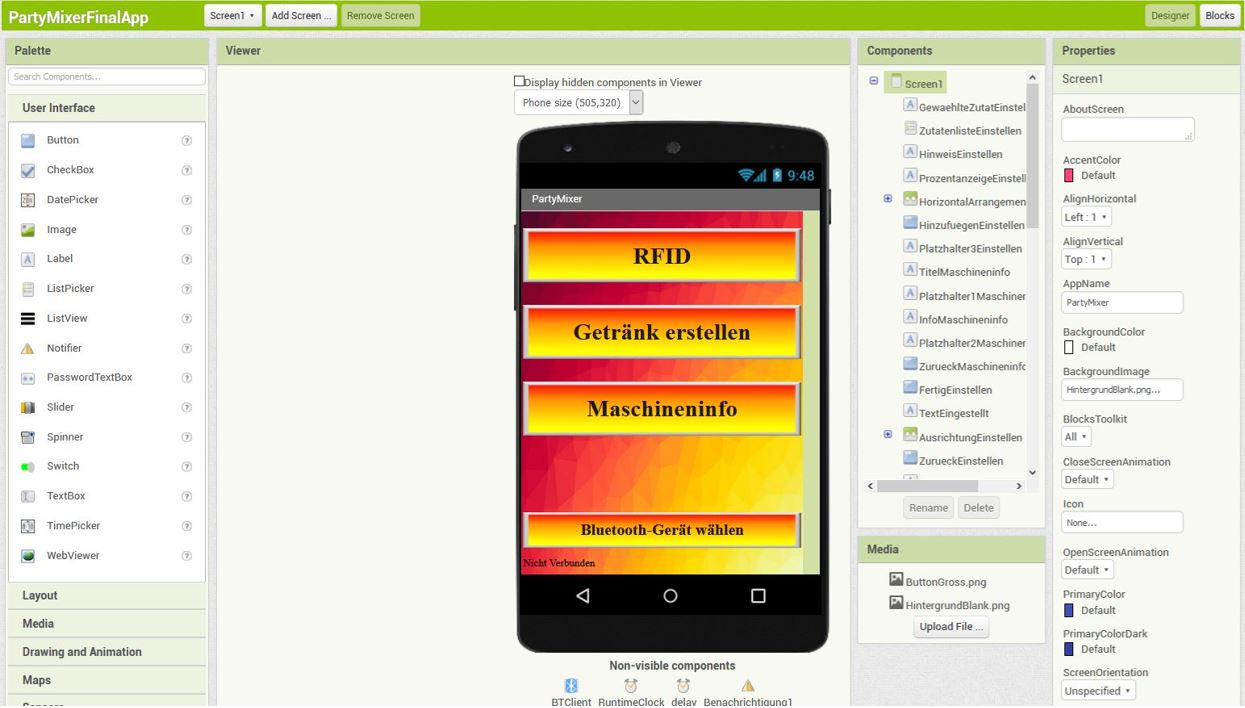
\includegraphics[width=\textwidth]{graphics/AppInventorDesigner}
	\caption{Designer von AppInventor \cite{appinventor_mit_nodate}}
	\label{fig:AppInventorDesigner}
\end{figure}

In den Blocks gemäss Abbildung \ref{fig:AppInventorBlocks} wird der eigentliche Programmablauf erstellt. Dabei ist der Programmablauf jedoch nicht handschriftlich zu erstellen, sondern kann mittels Blöcke zusammengesetzt werden. Dies erfordert zwar auch eine gewisse Programmierkenntnis, ist jedoch einfacher zu verstehen. Ausserdem sind viele Hilfeleistungen gegeben. Ein wichtiger Knackpunkt sind jedoch wie bei fast allen Programmiersprachen die Datentypen, welche sauber deklariert werden müssen.

\begin{figure}[h!]
	\centering
	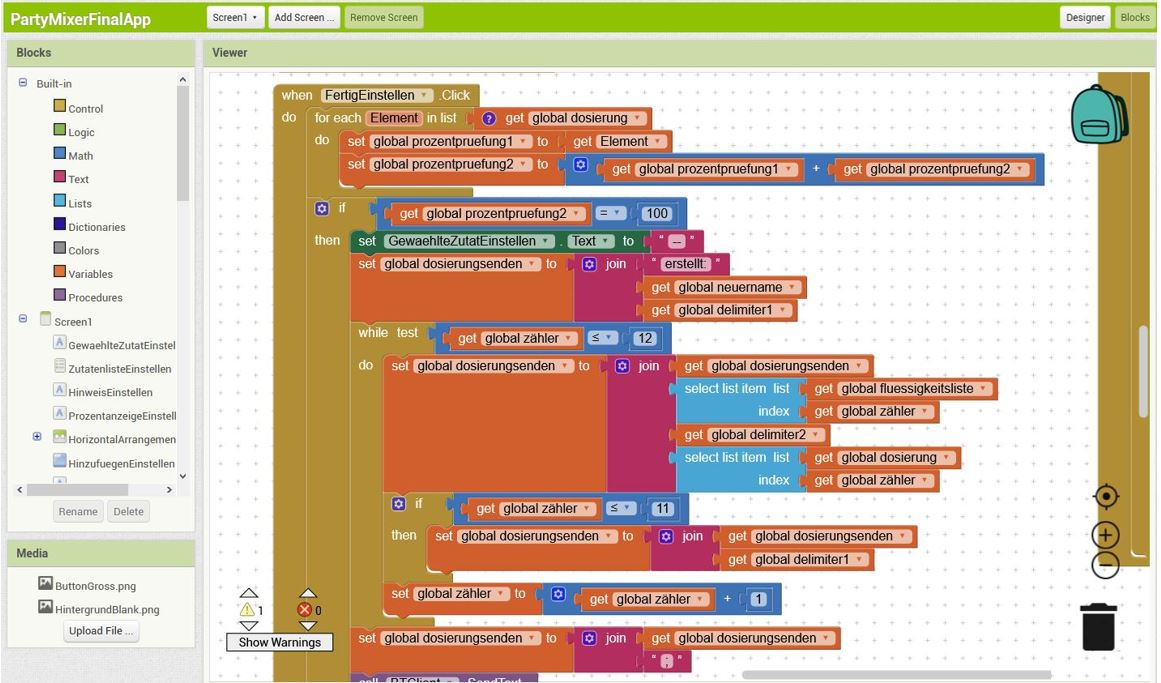
\includegraphics[width=\textwidth]{graphics/AppInventorBlocks}
	\caption{Blocks von AppInventor \cite{appinventor_mit_nodate}}
	\label{fig:AppInventorBlocks}
\end{figure}

Die App funktioniert auf allen Android-Geräten, welche den Grossteil des weltweiten Marktes ausmachen. AppInventor ist jedoch an einer Kooperation mit Apple dran, um die erstellten App's auch auf iOS benutzen zu können. Dies befindet sich momentan in der Betaphase. Somit sollte die App in naher Zukunft auch auf iOS verfügbar sein können. \cite{appinventor_mit_nodate-1}




 
